\documentclass[11pt]{article}

\usepackage[a4paper,margin=2.5cm]{geometry}
\usepackage{graphicx}
\usepackage{setspace}
\usepackage{caption}
\usepackage{float}
\usepackage{amsmath}
\usepackage{booktabs}
\usepackage{placeins}
\usepackage{url}
\usepackage{microtype}
\usepackage[numbers,sort&compress]{natbib}
\usepackage[hidelinks]{hyperref}

\captionsetup{font=small,labelfont=bf,labelsep=period}
\setlength{\parskip}{0.25em}
\setlength{\parindent}{1.5em}
\setlength{\textfloatsep}{0.9em plus 0.2em minus 0.2em}
\setlength{\floatsep}{0.9em plus 0.2em minus 0.2em}
\setlength{\intextsep}{0.9em plus 0.2em minus 0.2em}
\renewcommand{\topfraction}{0.92}
\renewcommand{\bottomfraction}{0.85}
\renewcommand{\textfraction}{0.08}
\renewcommand{\floatpagefraction}{0.80}
\setcounter{topnumber}{3}
\setcounter{bottomnumber}{2}
\setcounter{totalnumber}{5}
\emergencystretch=2em
\raggedbottom
\setstretch{1.20}

\begin{document}
\pagestyle{plain}

\begin{center}
{\LARGE\bfseries Repeatable station terms modify fixed-probability long-period response spectra at stations across Japan\par}
\vspace{0.6em}
{\large Haoyu Zhou\textsuperscript{1} and Qiang Ma\textsuperscript{1,*}\par}
\vspace{0.3em}
{\small \textsuperscript{1}Institute of Engineering Mechanics, China Earthquake Administration, 29 Xuefu Road, Nangang District, Harbin 150080, China\par}
{\small \textsuperscript{*}Correspondence: maqiang@iem.ac.cn\par}
{\small ORCID: Haoyu Zhou, 0009-0003-8817-1209; Qiang Ma, 0000-0002-9768-5223\par}
\end{center}

\vspace{0.8em}

\noindent\textbf{Abstract}

Regional ground-motion models describe average shaking, while repeatable station-specific residuals can change long-period response spectra. Here we analyse 222,664 Japanese surface records and separate earthquake and station contributions to residuals from a regional model. At 3.0 s, station terms estimated from independent earthquake groups correlate at 0.890. A relation calibrated with earlier K-NET records reduces error for later KiK-net station terms by 19.4\%. The cross-period shapes of surface-to-borehole response-spectrum ratios and station terms correlate at 0.635, and directional analyses identify repeatable path-dependent patterns. At 5.0 s, the crustal station pattern correlates at 0.304 with an independent Kanto simulation. Cross-validated station adjustments have a 5th--95th percentile interval of 0.624--1.338 and shift fixed-probability J-SHIS spectra in both directions. Station-level uncertainty remains large. European-Mediterranean records reproduce station-term stability, although the Japanese parameter relation does not transfer. Local spectral adjustment requires records representative of the target region and source-path distribution.

\section{Introduction}

Regional ground-motion models assign a common median to recordings with similar source, path and site descriptors. Repeated recordings at the same station often remain systematically above or below that median, motivating nonergodic source, site and path terms\cite{anderson1999,stewart2017,lavrentiadis2023,kuehn2019,kuehn2023}. Fully nonergodic models for Japan already resolve spatially varying source, site and path adjustments, and three-dimensional simulations provide an additional constraint on basin-related site terms\cite{sung2024,sung2025}.

Japan offers an unusually dense test of station-specific residuals. The J-SHIS/NIED Strong Ground Motion Flat File links K-NET and KiK-net records to earthquake sources, distances and site metadata\cite{niedflatfile,morikawa2024flatfile,kinoshita1998,aoi2004,aoi2020}. The Morikawa--Fujiwara 2013 model, hereafter MF2013, includes a magnitude-distance backbone and site terms based on AVS30 and D1400\cite{morikawa2013,morikawa2023}. AVS30 is the average shear-wave velocity in the upper 30 m, and D1400 is the depth to the 1.4 km s$^{-1}$ shear-wave velocity horizon. Their period-dependent coefficients provide a direct test of shallow-soil and deep-sedimentary contributions.

Long-period motion is sensitive to sedimentary depth and basin geometry. Observations and simulations in Japan show persistent amplification and surface-wave effects at periods relevant to large basins and long-period structures\cite{koketsu2008,yoshimoto2014,takemura2015,furumura2007}. A station residual in this band can combine local response, unresolved path structure and sensor effects. Japan's provisional probabilistic response-spectrum maps provide an engineering-bedrock coordinate on which such a correction can be tested\cite{dohi2024}.

We estimate event-adjusted station terms from MF2013 residuals and test their stability across independent earthquake groups, recording networks, a second ground-motion model and the European-Mediterranean archive\cite{esm2026}. KiK-net surface-to-borehole response-spectrum ratios, path-stratified records and an independent Kanto simulation constrain their physical interpretation\cite{sung2025}. The station terms are repeatable, retain both site-response and average-path contributions, and can be estimated partly from public site and regional parameters. Cross-validated adjustments modify matched J-SHIS long-period spectral accelerations in both directions, while source-class and regional tests delimit where those adjustments can be applied.

\section{Results}

\subsection{Surface-record residuals}

The public subset contains 333,808 records, of which 231,380 are from ground-surface installations; the remainder includes KiK-net borehole sensors. Requiring the MF2013 inputs leaves 222,664 records from 1,880 surface stations and 1,737 earthquakes at each period. Among these stations, 1,628 have at least 20 records and enter the station-level analysis. Their distribution covers the Japanese islands, and the earthquake set includes crustal, interplate and intraplate sources (Fig. \ref{fig:overview}a).

The D1400 and AVS30 terms improve the residual fit most strongly between 1 and 3 s. Their reduction in mean absolute residual is 3.0\% at 0.1 s and 14.0\% at 1.0 s, reaches 20.0\% and 21.4\% at 2.0 and 3.0 s, and decreases to 16.2\% at 5.0 s (Fig. \ref{fig:overview}b; Table \ref{tab:periods}; Supplementary Table 1). Every period is read directly from the flatfile RotD100 spectrum.

For each period, a two-way fixed-effects decomposition separates the residual into a global intercept, a between-event residual, a site-to-site residual and a remaining within-site residual. We refer to the site-to-site residual as the station term. Its dispersion is larger at short periods and decreases towards 5.0 s, while the between-event and within-site components vary less across period (Fig. \ref{fig:overview}c). The global intercept is retained as a model offset and is excluded from the station adjustment.

\begin{figure}[!htbp]
\centering
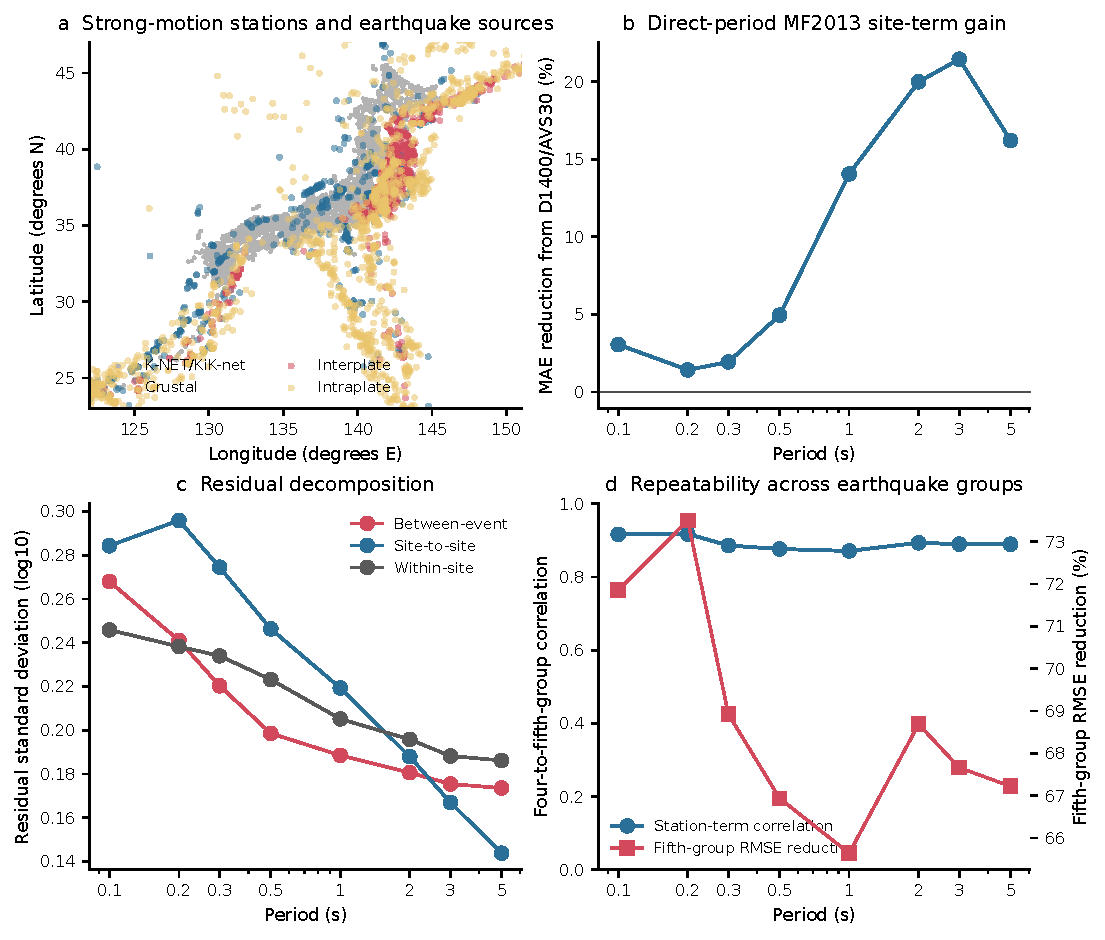
\includegraphics[width=0.98\linewidth]{figures/figure_event_adjusted_overview.pdf}
\caption{Data coverage and residual decomposition. \textbf{a}, K-NET and KiK-net stations and earthquake sources used in the residual calculation. \textbf{b}, Reduction in mean absolute residual after adding the MF2013 D1400 and AVS30 terms at directly observed periods. \textbf{c}, record-weighted standard deviations of the between-event and site-to-site residuals and the root mean squared within-site residual. \textbf{d}, repeatability of station terms across five independent earthquake groups. Blue circles show the mean correlation between terms estimated from four groups and the fifth group; red squares show the mean reduction in fifth-group root mean squared error relative to the zero-station-term baseline.}
\label{fig:overview}
\end{figure}

\subsection{Station terms recur across events}

Station terms estimated from disjoint earthquake groups remain strongly correlated. Each comparison estimates one set of terms from four groups and a second set from the fifth group. At 3.0 s, the fifth group contains about 347 earthquakes, and an average of 1,481 stations meet both record thresholds. The mean correlation between the two sets is 0.890. Using the four-group terms to estimate the fifth-group terms reduces root mean squared error by 67.7\% relative to zero. Correlations range from 0.871 to 0.917 across 0.1--5.0 s, and the period-specific reductions range from 65.6\% to 73.5\% (Fig. \ref{fig:overview}d; Supplementary Fig. 1; Supplementary Table 2).

The MF2013 site terms remove most of the long-period association with D1400. At 3.0 s, the event-adjusted station correlation with D1400 decreases from 0.751 for the magnitude-distance backbone to 0.194 after the D1400 and AVS30 terms are added (Fig. \ref{fig:structure}a,c). The corresponding correlation with basement depth decreases but remains positive (Fig. \ref{fig:structure}b). The station terms retain basin-related or other spatial structure beyond the two MF2013 site variables.

An approximate application of the MF2013 anomalous-intensity term changes individual residuals but preserves the spatial pattern of the station terms. At 3.0 s, primary and sensitivity station terms correlate at 0.971, and the D1400 correlation changes from 0.194 to 0.206 (Fig. \ref{fig:structure}d). The main period pattern is insensitive to this approximation.

\begin{figure}[!htbp]
\centering
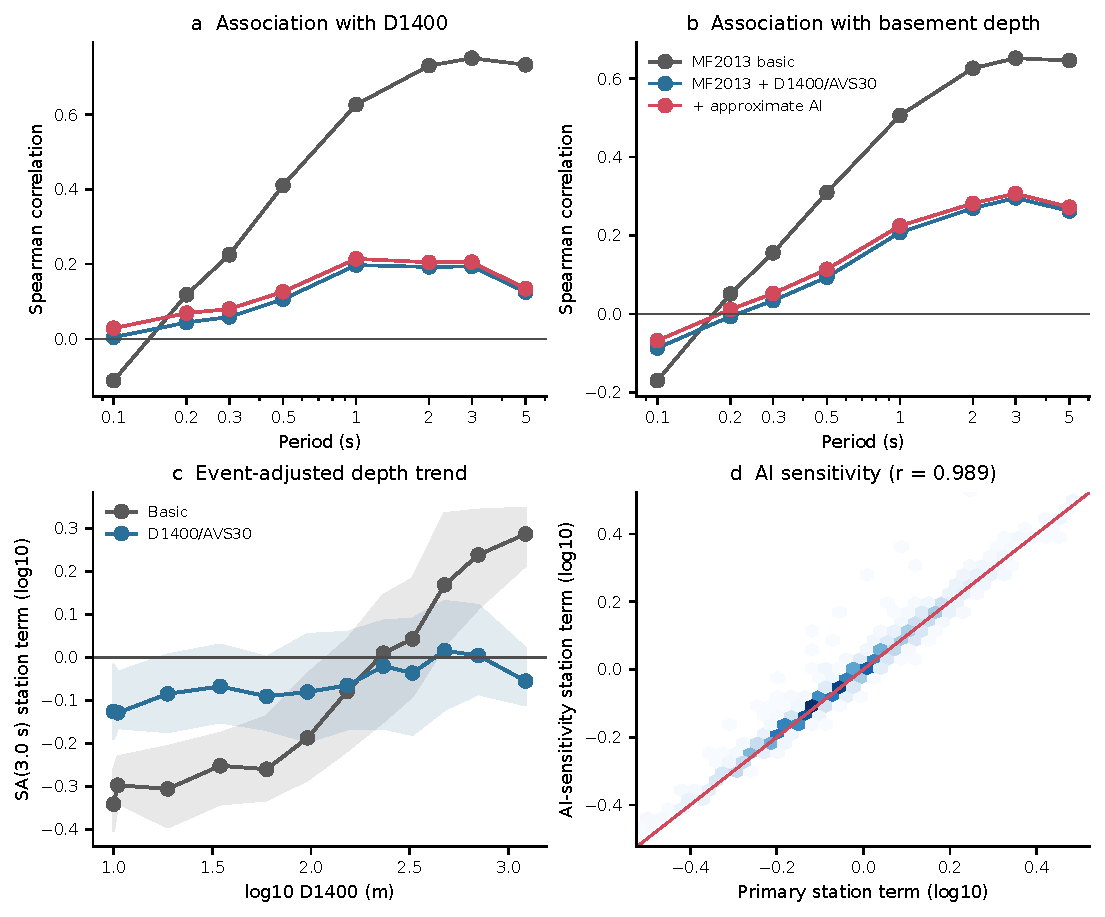
\includegraphics[width=0.98\linewidth]{figures/figure_event_adjusted_site_structure.pdf}
\caption{Event-adjusted station terms and sedimentary-depth variables. \textbf{a}, Spearman correlations between station terms and D1400. \textbf{b}, correlations with basement depth. Grey denotes the MF2013 magnitude-distance backbone, blue includes D1400 and AVS30, and red adds the rule-based anomalous-intensity sensitivity. \textbf{c}, binned SA(3.0 s) station terms against D1400 before and after the site terms; lines show bin medians and bands show interquartile ranges. \textbf{d}, comparison between primary and anomalous-intensity sensitivity station terms at 3.0 s; the dashed diagonal marks equality.}
\label{fig:structure}
\end{figure}

\subsection{Station patterns persist under a second model}

We repeated the residual decomposition with the Zhao et al. 2006 model as implemented in OpenQuake\cite{zhao2006,pagani2014}. The source-class-specific active-crustal, interface and intraslab variants use the same surface observations, source classes, AVS30 values and documented shortest fault distances. At 3.0 s, the MF2013 and Zhao station terms correlate at 0.770 across 1,628 stations; the record-weighted correlation is 0.735, and the median absolute difference is 0.151 log$_{10}$ units (Fig. \ref{fig:independent}; Supplementary Table 3). Their signs agree at 77.5\% of stations. Correlations decrease from 0.953 at 0.1 s to 0.697 at 5.0 s, showing greater backbone dependence at long periods while retaining a common spatial ordering.

The Zhao residuals also repeat across independent earthquake groups. Their 3.0 s station-term correlation is 0.950, and the site-and-regional-parameter model reduces spatial-block root mean squared error by 37.7\%, with a record-derived versus estimated correlation of 0.792. Both calculations use the same observations and validation design, so this comparison measures sensitivity to the ground-motion model.

\begin{figure}[!htbp]
\centering
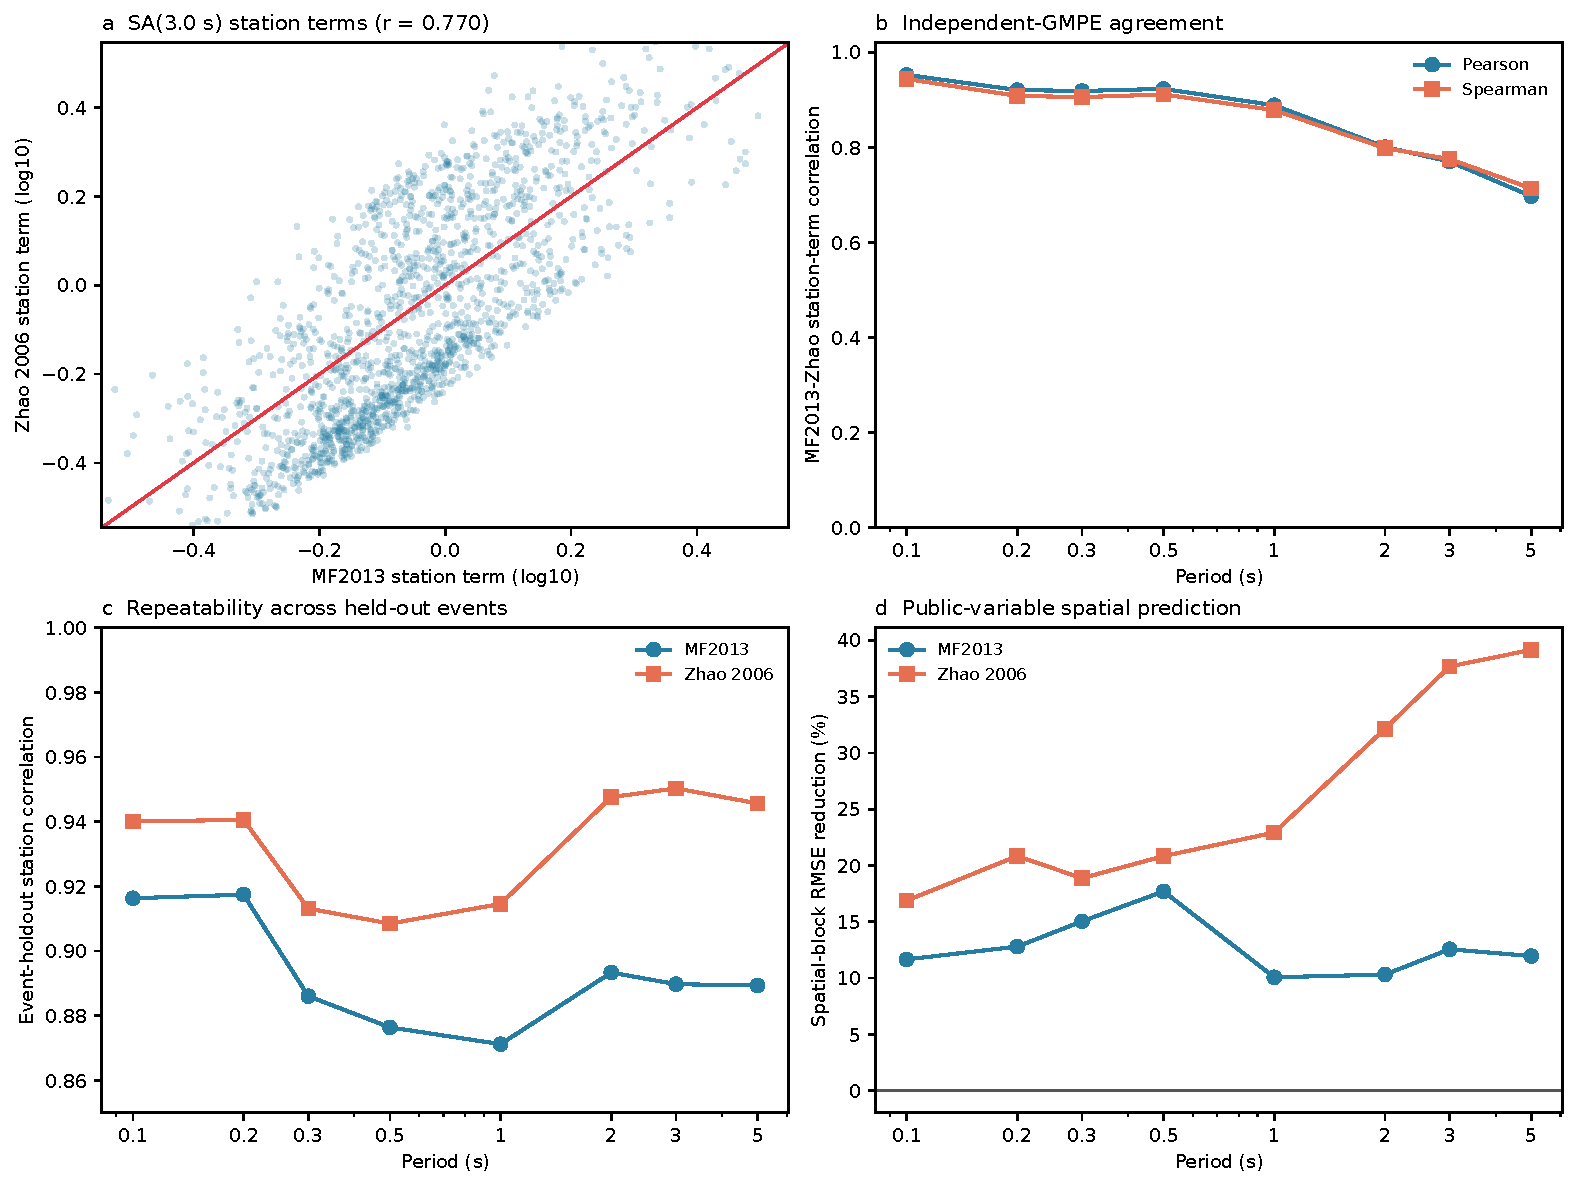
\includegraphics[width=0.96\linewidth]{figures/figure_ground_motion_model_sensitivity.pdf}
\caption{Ground-motion-model sensitivity of the station-term pattern. \textbf{a}, MF2013 and Zhao 2006 station terms at 3.0 s; the dashed diagonal marks equality. \textbf{b}, station-term correlations across the eight direct periods. \textbf{c}, event-group repeatability for both residual models. \textbf{d}, spatial-block root mean squared error reduction for the site-and-regional-parameter model. Both residual calculations use the same surface records.}
\label{fig:independent}
\end{figure}

\subsection{Paired surface and borehole spectra support site response}

The flatfile contains 102,428 KiK-net event--site pairs with positive surface and borehole RotD100 ordinates at each analysed period, covering 699 sites and 1,410 earthquakes. Among 639 sites linked to supported primary station terms, the station term and median surface--borehole ratio at 3.0 s have Pearson and Spearman correlations of 0.315 and 0.415. Removing linear trends with log borehole depth gives a Pearson correlation of 0.327. The Pearson correlation is 0.737 at 0.1 s, 0.522 at 1.0 s and 0.395 at 2.0 s (Supplementary Fig. 2; Supplementary Table 4).

The paired response-spectrum ratios are stable across independent earthquake groups. At 3.0 s, their mean correlation between estimation and test groups is 0.988. A relation calibrated from estimation-group ratios and station terms estimates station terms derived independently from the test earthquakes with a mean correlation of 0.290 and a 2.7\% root mean squared error reduction relative to the no-station-adjustment baseline. Cross-period behaviour provides stronger evidence: after removing each station's mean amplitude and the network-wide period mean, the shapes of the surface-to-borehole ratios and station terms correlate at 0.677 across all earthquakes. Across five tests that use disjoint earthquake groups for the two quantities, the correlations remain 0.597--0.670, with a mean of 0.635. The median within-station spectral-shape correlation is 0.769, and 91.5\% of stations have a positive value (Supplementary Fig. 3; Supplementary Table 17).

\subsection{Cross-network estimates remain stable through time}

We next separated recording network and earthquake sample simultaneously. Of 1,286 earthquakes represented by at least five records in each network, K-NET station terms from four earthquake groups define the parameter relation; KiK-net station terms from the fifth group provide an independent comparison. At 3.0 s, the site-parameter model estimates terms for 677 KiK-net stations with a correlation of 0.439 and a 13.0\% root mean squared error reduction. Adding regional parameters raises these values to 0.598 (station-bootstrap 95\% interval 0.542--0.651) and 20.8\% (13.3--26.7\%). Both relations are fitted and centred with K-NET data from the four earthquake groups.

The K-NET-to-KiK-net correlation is 0.543--0.642 across the eight periods, and every period reduces error by 18.5\%--25.9\%. The reverse calculation uses the smaller KiK-net sample to estimate K-NET terms from an independent earthquake group. At 3.0 s it gives a correlation of 0.462 and a 4.0\% error reduction; the latter has a bootstrap interval of $-0.8\%$ to 8.8\%. This asymmetry identifies source-network record coverage as a constraint on cross-network application (Fig. \ref{fig:network}; Supplementary Table 18).

Chronological separation gives a similar result. Among 1,277 common earthquakes with finite origin times, the earliest 80\% end on 22 November 2016 and supply K-NET estimation terms; the latest 20\% begin on 24 November 2016 and supply independent KiK-net terms. At 3.0 s, the fixed relation estimates terms for 547 stations represented by 256 later earthquakes with a correlation of 0.536 (95\% interval 0.469--0.600) and a 19.4\% root mean squared error reduction (13.6--24.9\%). The 80/20 result remains positive at all eight periods, with correlations of 0.460--0.635 and error reductions of 12.6\%--21.5\%. Results at 1--3 s also remain positive under 70/30 and 90/10 time splits. Reversing the 80/20 calculation gives a 3.0 s correlation of 0.302 and increases error by 3.3\%; its error-reduction interval is $-7.8\%$ to 1.5\% (Supplementary Table 20).

\begin{figure}[!htbp]
\centering
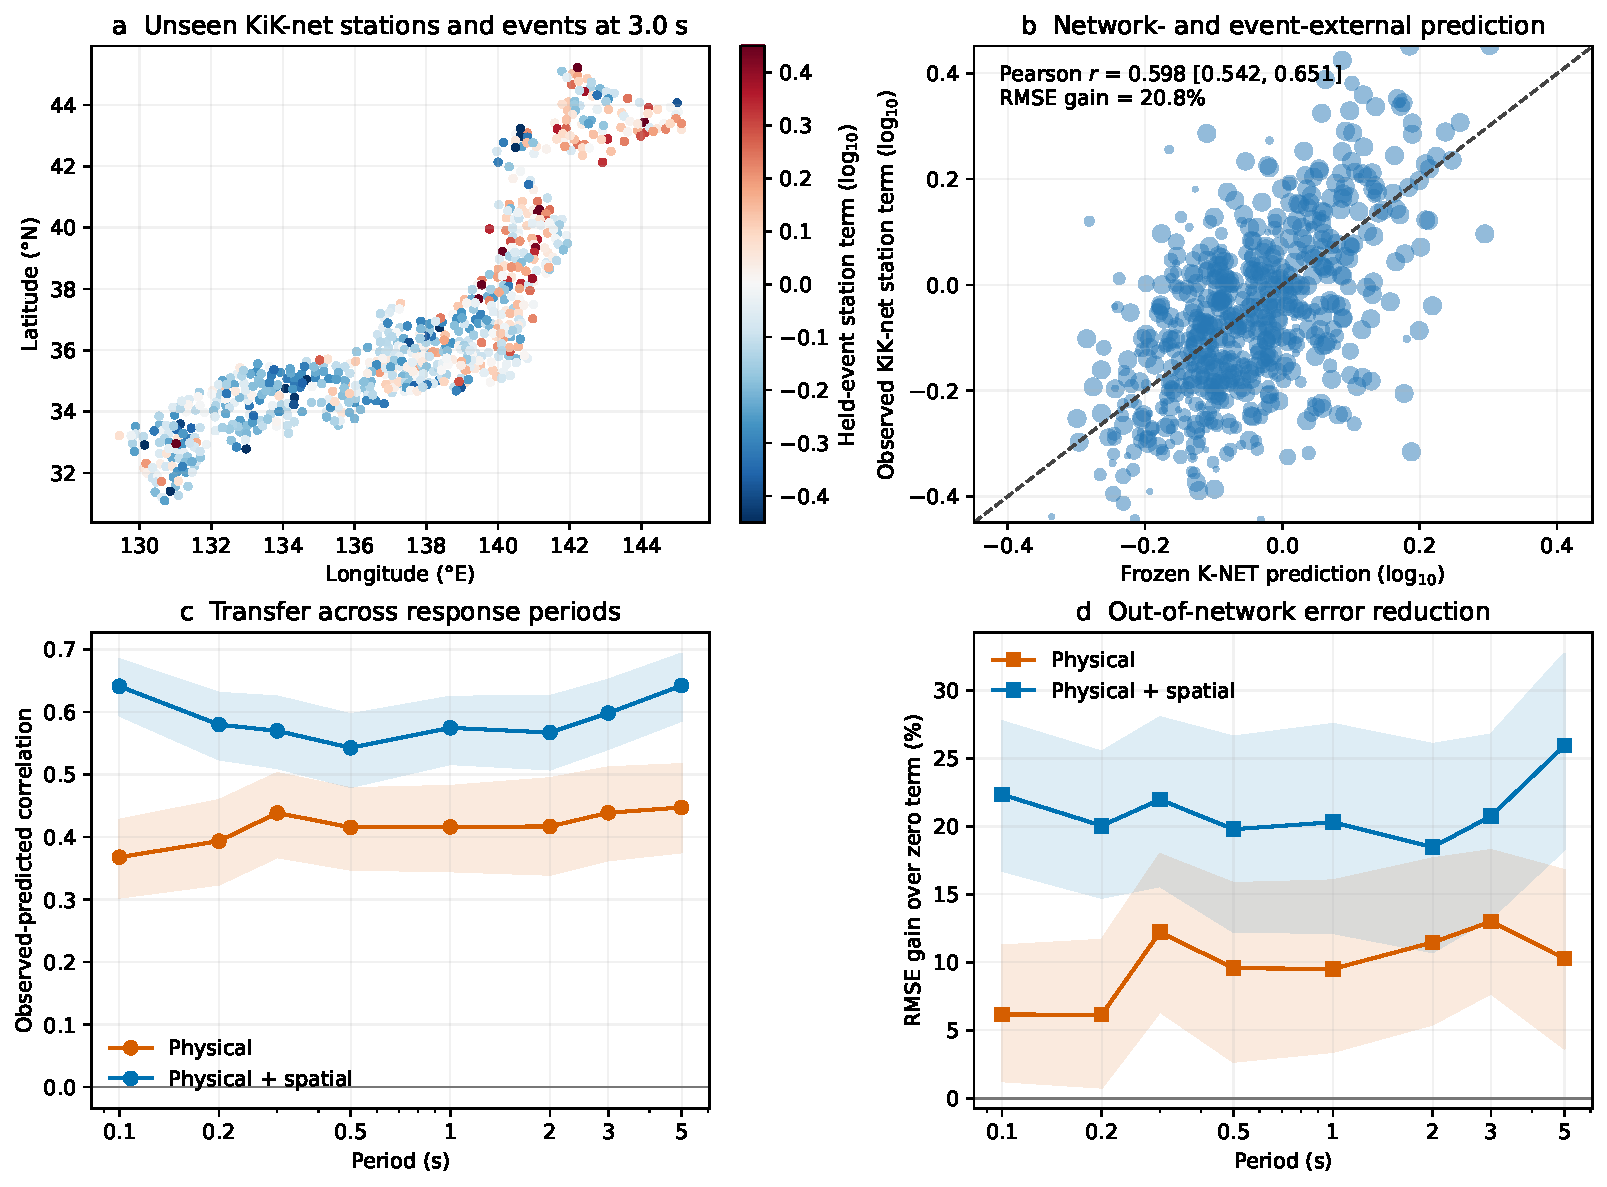
\includegraphics[width=0.98\linewidth]{figures/figure_cross_network_transfer_validation.pdf}
\caption{Cross-network station-term estimation with independent earthquake groups. \textbf{a}, KiK-net stations whose terms are derived from the fifth earthquake group at 3.0 s. \textbf{b}, K-NET-based estimates against record-derived KiK-net station terms; point area scales with fifth-group record count and the dashed diagonal marks equality. \textbf{c}, correlations for the site-parameter and site-and-regional-parameter models across period; bands are station-bootstrap 95\% intervals. \textbf{d}, root mean squared error reduction relative to the zero-station-term baseline.}
\label{fig:network}
\end{figure}

\subsection{European records reproduce station recurrence}

We next tested station recurrence outside Japan using version 3 of the Engineering Strong-Motion database. The primary sample contains 13,430 records from 634 shallow European-Mediterranean earthquakes that occurred from 2015 onwards, after publication of the fixed Bindi et al. model\cite{esm2026,bindi2014}. Residuals use the as-recorded horizontal geometric-mean spectrum at 1.0, 2.0 and 3.0 s. Among 265 stations with at least 15 records, the mean correlations between station terms fitted to independent earthquake groups are 0.929, 0.939 and 0.928. Their station-bootstrap 95\% intervals are 0.899--0.950, 0.915--0.957 and 0.896--0.951, and the corresponding root mean squared error reductions are 66.8\%, 69.5\% and 66.4\% (Fig. \ref{fig:esm}; Supplementary Table 21).

The result remains positive after raising the minimum magnitude to $M_w=5$: correlations are 0.871--0.878 and error reductions are 52.2\%--53.4\%. A Kotha et al. model with RotD50 gives correlations of 0.860--0.919 in a smaller sample\cite{kotha2020}. The 3.0 s station-term standard deviation is 0.243 log$_{10}$ units in ESM and 0.168 log$_{10}$ units in Japan. A fixed K-NET relation restricted to the two harmonised variables, log$_{10}(V_{S30})$ and elevation, does not reproduce the ESM station terms after aligning the predicted mean without using ESM residuals: at 3.0 s its correlation is 0.047 and its error reduction is $-2.8\%$. Station terms recur outside Japan, but their relation to public site variables remains region dependent.

Local ESM estimation gives the same spatial boundary. The test retains 236 stations in the largest connected component; a fixed minimum of 30 stations per block selects three geographic blocks without using response values. At 3.0 s, the locally fitted $V_{S30}$--elevation model gives a correlation of 0.074 and an error reduction of $-3.6\%$ (95\% interval $-9.8\%$ to 1.3\%). Adding the available ESM site metadata and coordinates gives a correlation of 0.017 and an error reduction of $-7.6\%$ ($-13.1\%$ to $-2.2\%$). A stricter test fits four earthquake groups outside one spatial block and evaluates fifth-group station terms inside that block; its $V_{S30}$--elevation correlation is 0.021 and its error reduction is $-3.7\%$ ($-8.6\%$ to 0.5\%). Every aggregate spatial error reduction at 1--3 s is negative (Supplementary Table 22).

\begin{figure}[!htbp]
\centering
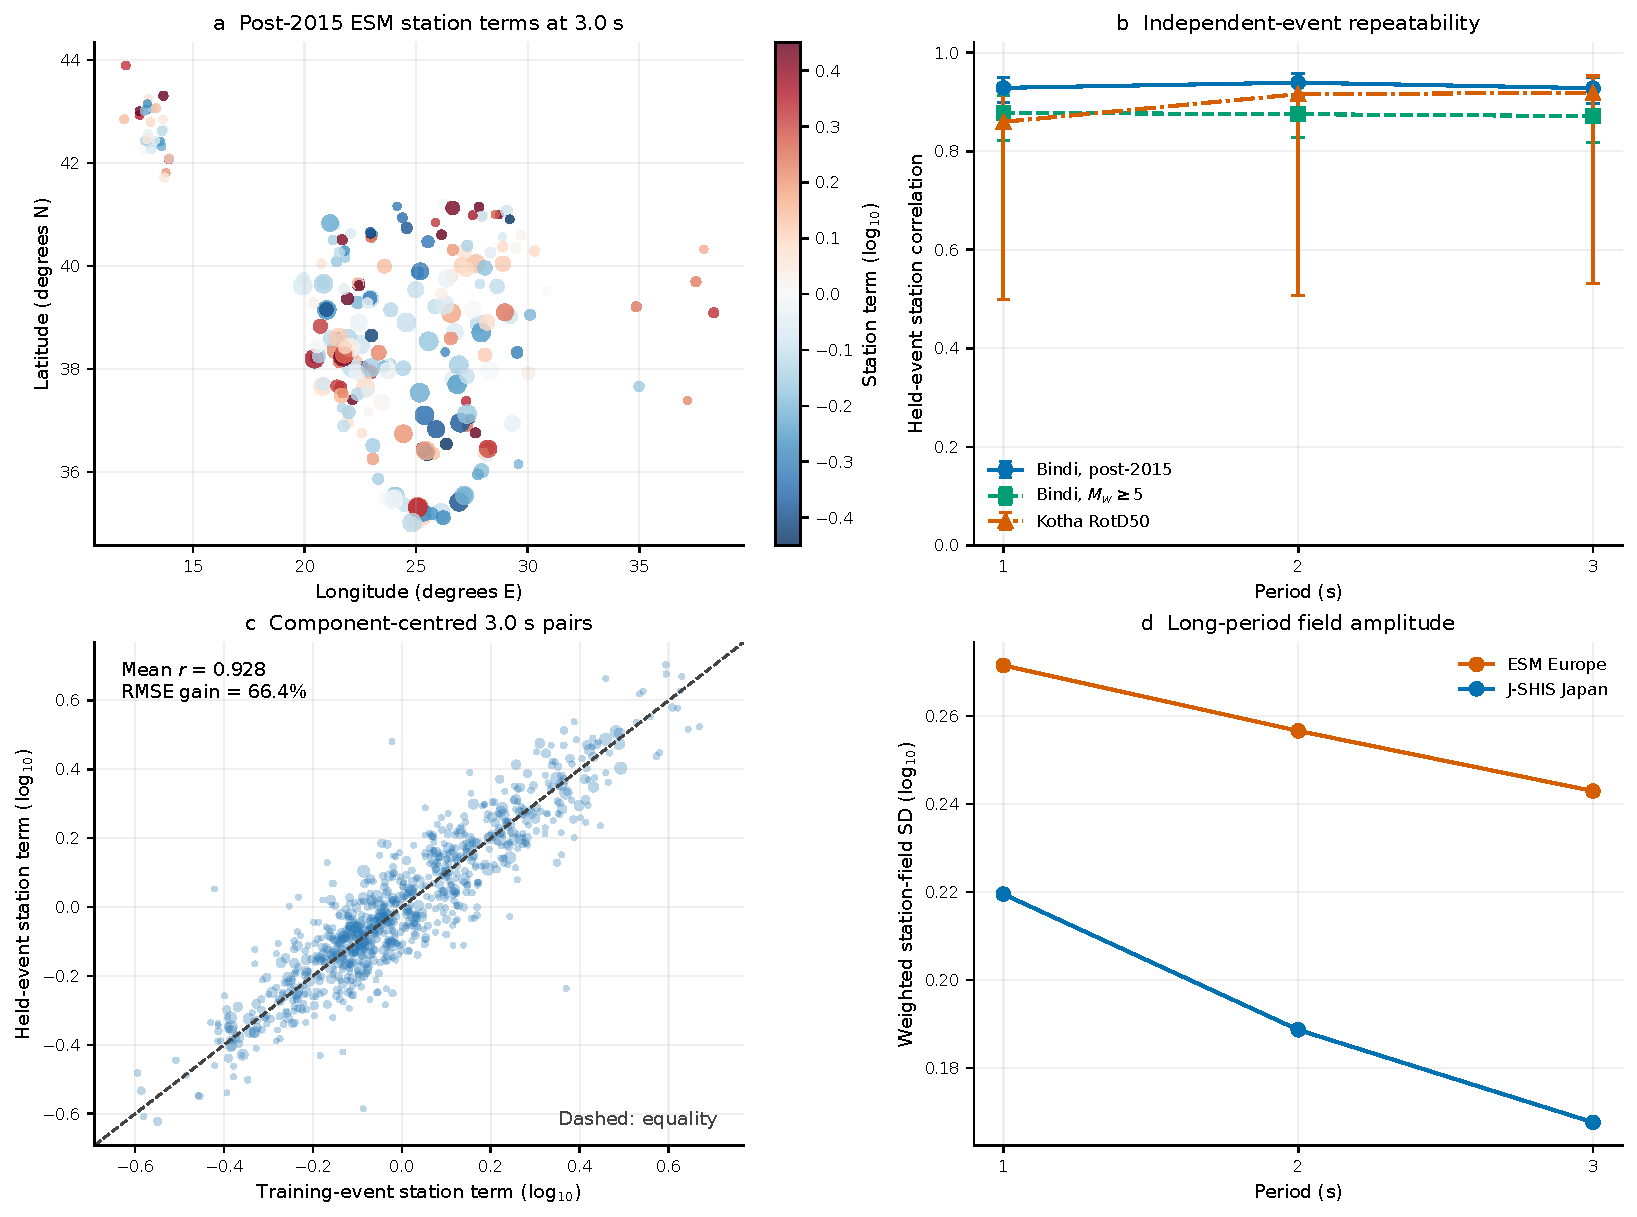
\includegraphics[width=0.98\linewidth]{figures/figure_esm_external_validation.pdf}
\caption{Independent European-Mediterranean station-term validation. \textbf{a}, post-2015 ESM station terms at 3.0 s; symbol area scales with station record count. \textbf{b}, mean correlations between station terms from independent earthquake groups; bars show station-bootstrap 95\% intervals. \textbf{c}, component-centred four-group and fifth-group station terms for the primary 3.0 s analysis; symbol area scales with fifth-group record count and the dashed diagonal marks equality. \textbf{d}, record-weighted station-term standard deviations in ESM and Japan.}
\label{fig:esm}
\end{figure}

\begin{table}[!htbp]
\centering
\caption{Residual and spatial-estimation results at direct periods}
\label{tab:periods}
\small
\begin{tabular}{rrrrrr}
\toprule
Period & MAE gain & \multicolumn{2}{c}{D1400 correlation} & Event-group & Spatial RMSE \\
(s) & (\%) & Basic & Site & correlation & gain (\%) \\
\midrule
0.1 & 3.0 & -0.112 & 0.004 & 0.916 & 11.7 \\
0.2 & 1.4 & 0.118 & 0.044 & 0.917 & 12.8 \\
0.3 & 1.9 & 0.225 & 0.059 & 0.886 & 15.0 \\
0.5 & 4.9 & 0.411 & 0.106 & 0.876 & 17.7 \\
1.0 & 14.0 & 0.627 & 0.198 & 0.871 & 10.1 \\
2.0 & 20.0 & 0.731 & 0.192 & 0.893 & 10.3 \\
3.0 & 21.4 & 0.751 & 0.194 & 0.890 & 12.6 \\
5.0 & 16.2 & 0.733 & 0.125 & 0.889 & 12.0 \\
\bottomrule
\end{tabular}
\end{table}

\subsection{Site and regional parameters explain station terms}

The site-parameter model uses shallow velocities, sedimentary depths, elevation, sensor depth and recording network. At 3.0 s its spatial-block root mean squared error is 2.3\% higher than the no-station-adjustment baseline. Adding longitude, latitude and volcanic-front distances defines the site-and-regional-parameter model, which reduces error by 12.6\% and gives a correlation of 0.500 between record-derived and estimated station terms. Error reductions across the five test blocks range from 10.2\% to 34.1\%. Site descriptors retain associations with the residuals, and station location adds information on regional structure and average path coverage.

The site-and-regional-parameter model improves on the no-adjustment baseline at every direct period. Root mean squared error reductions are 10.1\%, 10.3\%, 12.6\% and 12.0\% at 1.0, 2.0, 3.0 and 5.0 s, respectively (Fig. \ref{fig:hazard}b; Supplementary Fig. 4; Supplementary Table 5). Fixed macroregion tests are less uniform: the full model improves all five regions by 5.4\% to 28.9\%, whereas the common-feature sensitivity changes from $-5.2\%$ to 27.5\% (Supplementary Fig. 5; Supplementary Table 6). Joint deletion of the ten highest-count earthquakes leaves station-term correlations above 0.9989 at every period and changes the 3.0 s terms by 0.012 log$_{10}$ units at their record-weighted 95th percentile (Supplementary Table 7).

Across six fixed model-complexity settings, the 3.0 s error reduction remains between 10.5\% and 14.0\%. Every setting improves on the no-adjustment baseline at all eight periods, with gains from 7.1\% to 19.3\%. The primary settings remain fixed, and the alternatives quantify model sensitivity.

The primary analysis uses the full domain of the public flatfile. Applying the complete published MF2013 regression-domain screens, including the Kanno-PGA distance cutoff, leaves 35,857 records from 411 earthquakes\cite{kanno2006}. At 3.0 s, station-term patterns from the restricted and primary samples correlate at 0.959 across 578 supported stations. Within the restricted sample, independent earthquake groups correlate at 0.762, and the site-and-regional-parameter model reduces spatial-block error by 4.1\%. The gain is positive from 0.2 to 5.0 s and is $-2.3\%$ at 0.1 s.

\begin{figure}[!htbp]
\centering
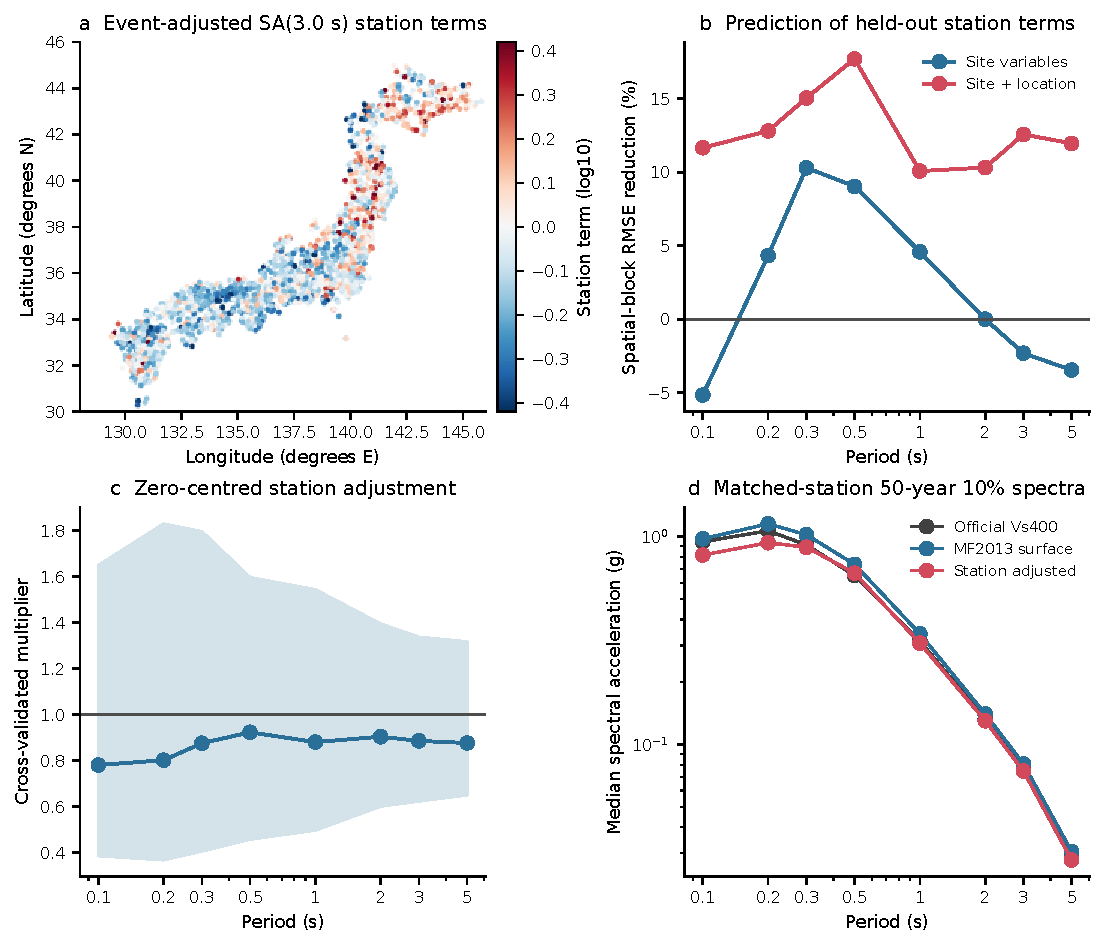
\includegraphics[width=0.98\linewidth]{figures/figure_event_adjusted_multiperiod.pdf}
\caption{Station-term spatial estimation and response-spectrum adjustment. \textbf{a}, event-adjusted SA(3.0 s) station terms at stations with at least 20 records. \textbf{b}, spatial-block root mean squared error reduction for the site-parameter and site-and-regional-parameter models. \textbf{c}, median and 5th--95th percentile range of zero-centred cross-validated station multipliers. \textbf{d}, matched-station median response spectra at the 50-year 10\% exceedance probability on J-SHIS $V_S=400$ m s$^{-1}$ engineering bedrock, after conversion to the station surface condition, and after the station adjustment. All periods are calculated directly.}
\label{fig:hazard}
\end{figure}

\subsection{Path strata reveal conditional station terms}

Random separation into earthquake groups preserves the broad path distribution sampled at each station. We re-estimated station terms within four hypocentral-bearing sectors, four shortest-fault-distance bins and the three source classes. At 3.0 s, source-class patterns correlate at 0.924--0.942 with the all-record pattern, and the 100--300 km distance patterns correlate at 0.963--0.974. Directional-sector correlations span 0.280--0.886, while within-component correlations between disjoint earthquake halves of the same sectors span 0.764--0.969 (Fig. \ref{fig:path}; Supplementary Table 8). High repeatability within a sector alongside low agreement with the all-record result identifies a systematic directional component.

Equal weighting across available path strata retains a weaker persistent component. At 1--3 s, models fitted to azimuth-, distance- and source-class-balanced station terms reduce overall spatial-block error by 2.5\%--9.6\%. Several individual spatial blocks have negative gains, including the azimuth-balanced 3.0 s result (Supplementary Fig. 6; Supplementary Table 9). Public station variables explain part of the residual pattern averaged over the sampled paths, and the strength of this relation varies with path coverage.

\begin{figure}[!htbp]
\centering
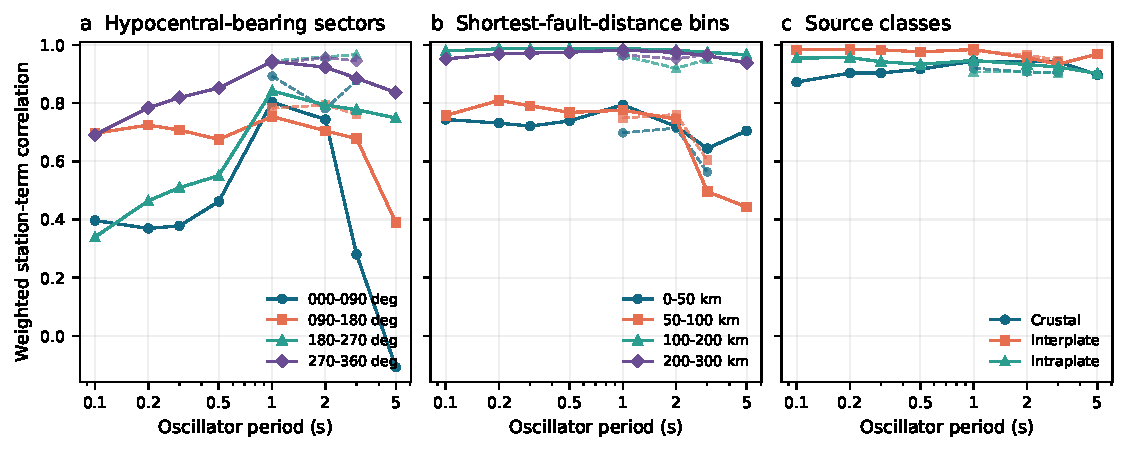
\includegraphics[width=0.98\linewidth]{figures/figure_path_stratification.pdf}
\caption{Path and source stratification of station terms. \textbf{a}, hypocentral-bearing sectors. \textbf{b}, shortest-fault-distance bins. \textbf{c}, source classes. Solid lines compare each stratum-specific pattern with the all-record pattern at all eight periods. Dashed lines show mean within-component correlations between five pairs of disjoint earthquake halves at 1.0, 2.0 and 3.0 s. Disconnected station--event graphs are solved separately; split-half correlations remove the weighted offset of every intersecting component pair.}
\label{fig:path}
\end{figure}

\subsection{Source class changes long-period spatial estimation}

Requiring 20 records within a source class retains 1,084 crustal, 779 interplate and 856 intraplate stations at each period. At 3.0 s, the fixed site-and-regional-parameter model gives record-derived versus estimated correlations of 0.455, 0.251 and 0.516 for these classes. The corresponding root mean squared error reductions are 8.9\% (95\% interval 3.9--13.8\%), 2.8\% ($-1.7\%$ to 7.4\%) and 14.3\% (10.1--18.3\%) (Supplementary Fig. 7; Supplementary Table 24).

At 5.0 s, the crustal and interplate reductions are 4.2\% ($-0.7\%$ to 8.9\%) and 1.7\% ($-2.8\%$ to 5.9\%), while the intraplate reduction is 14.8\% (10.7--18.6\%). The full period set retains a crustal reduction of $-8.6\%$ at 0.1 s and an interplate reduction of $-0.8\%$ at 2.0 s. Source class changes both the amplitude and the spatial estimability of the station terms.

The source-matched Kanto comparison uses the 5.0 s adjusted site-term distribution from the independent three-dimensional simulations of Sung et al.\cite{sung2025}. Across 364 matched stations, the record-derived crustal station terms have a Pearson correlation of 0.304 (31.7 km spatial-block 95\% interval 0.163--0.434), a Spearman correlation of 0.372 (0.227--0.494) and 62.9\% centred-sign agreement with the simulation result. The source-conditioned cross-validated estimate correlates at 0.135 (0.038--0.231); the all-source cross-validated estimate correlates at 0.349 (0.243--0.446) (Supplementary Fig. 8; Supplementary Table 25). The empirical and simulated patterns show a weak positive spatial association with substantial station-scale scatter. Public variables recover only part of that spatial variation.

\subsection{Station adjustments shift fixed-probability spectra}

The primary cross-validated station-term estimates are centred to zero in log space before application to the response spectra. At 3.0 s, their multipliers have 5th, 50th and 95th percentiles of 0.624, 0.886 and 1.338 (Fig. \ref{fig:hazard}c). The corresponding local changes are $-37.6\%$, $-11.4\%$ and $+33.8\%$. At 5.0 s, the 5th and 95th percentiles are 0.651 and 1.318.

The J-SHIS response-spectrum maps give spectral acceleration on engineering bedrock with $V_S=400$ m s$^{-1}$. At each matched station, we replace the MF2013 shallow-site factor for 400 m s$^{-1}$ with the factor for the station AVS30. At 3.0 s and a 10\% probability of exceedance in 50 years, the median engineering-bedrock spectral acceleration is 0.078 g and the median after conversion to the station surface condition is 0.081 g. Applying the cross-validated station multiplier changes the median to 0.075 g (Fig. \ref{fig:hazard}d; Supplementary Fig. 9; Supplementary Table 10). The global MF2013 residual offset is excluded from this station adjustment.

The strict-domain 3.0 s multipliers span 0.660--1.503 between their 5th and 95th percentiles. On the same 578 stations, the primary estimate changes the surface-spectrum median from 0.094 to 0.098 g, while the strict-domain estimate changes it to 0.096 g. Local upward and downward changes persist; the aggregate median depends on the record domain and station set.

Spatial-block errors provide a separate empirical estimation interval for each test block. At 3.0 s, nominal 80\% and 90\% intervals cover 77.9\% and 89.0\% of stations. They exclude a unit multiplier at 8.4\% and 2.0\% of stations, respectively. The 90\% interval has a median upper-to-lower multiplier span of 3.00. Uncertainty in individual station estimates is appreciable even though the point estimates change many local spectral accelerations.

An independent station-adjustment pattern is obtained from the fixed K-NET relation and KiK-net terms based on a disjoint earthquake group. At 3.0 s, this pattern and the primary spatial-block estimate correlate at 0.736 across 639 KiK-net sites, agree in direction at 79.7\%, and both exceed a 10\% change in the same direction at 57.9\%. Their median absolute difference is 0.053 log$_{10}$ units (Supplementary Fig. 10 and Supplementary Fig. 11; Supplementary Table 11 and Supplementary Table 19). Estimation intervals describe spatial-model error, whereas independent-model agreement measures reproducibility. Source recurrence, ground-motion-model and J-SHIS logic-tree uncertainties remain separate.

We apply the same all-source station adjustment separately to the J-SHIS active-shallow and subduction response-spectrum layers. At the 50-year 10\% level and 3.0 s, the subduction spectral acceleration is at least as large at 1,428 of 1,628 stations, while the active-shallow value is larger at 200. Their median engineering-bedrock values are 0.071 and 0.031 g; surface conversion and station adjustment change the medians to 0.067 and 0.029 g, respectively. The two layers are evaluated separately because fixed-probability hazard values do not add linearly (Supplementary Fig. 12; Supplementary Table 23).

A second sensitivity applies crustal station terms to the active-shallow layer and applies interplate and intraplate terms separately to the subduction layer. Their 3.0 s multiplier ranges between the 5th and 95th percentiles are 0.642--1.517, 0.711--1.430 and 0.661--1.416. The matched-station median changes from 0.034 to 0.033 g for active-shallow/crustal, from 0.082 to 0.084 g for subduction/interplate and from 0.089 to 0.083 g for subduction/intraplate (Supplementary Table 26). The two subduction sensitivities remain separate because official interplate and intraplate source weights are unavailable.

City-nearest matched stations illustrate the bidirectional effect. At 3.0 s, the cross-validated changes are $-2.5\%$ near Tokyo, $-11.5\%$ near Osaka, $+31.2\%$ near Sapporo, $-11.0\%$ near Sendai and $-25.2\%$ near Fukuoka (Fig. \ref{fig:cities}; Supplementary Table 12). Each value is a station-level example for the nearest analysed station.

\begin{figure}[!htbp]
\centering
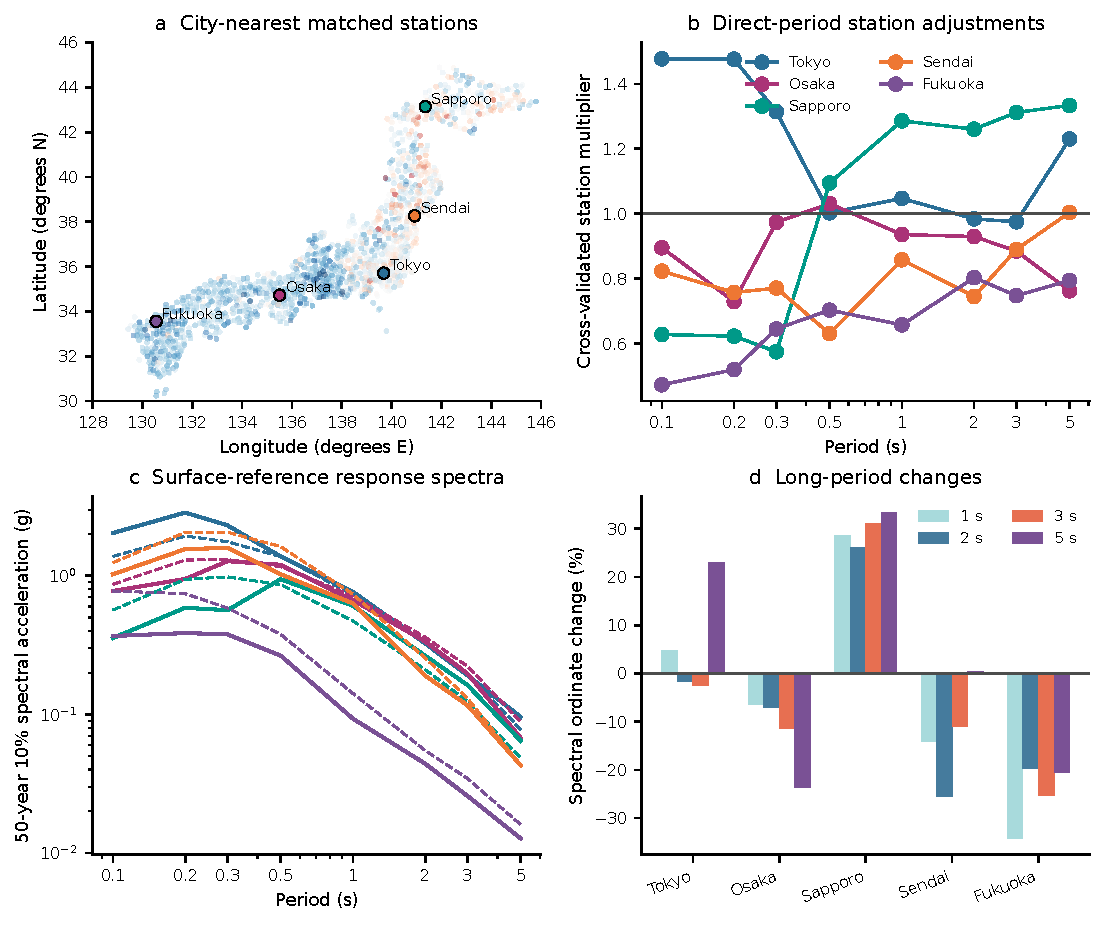
\includegraphics[width=0.72\linewidth]{figures/figure_event_adjusted_city_cases.pdf}
\caption{Illustrative city-nearest station cases. \textbf{a}, analysed stations nearest to five Japanese cities. \textbf{b}, direct-period cross-validated multipliers at the selected stations. \textbf{c}, surface-condition response spectra at the 50-year 10\% exceedance probability before and after the station adjustment; dashed and solid lines denote the two spectra. \textbf{d}, percentage changes at 1.0, 2.0, 3.0 and 5.0 s. Distances to the selected stations are 2.4 km for Tokyo, 3.6 km for Osaka, 8.6 km for Sapporo, 5.0 km for Sendai and 14.1 km for Fukuoka.}
\label{fig:cities}
\end{figure}

\section{Discussion}

The MF2013 AVS30 and D1400 terms remove most of the association between long-period residuals and shallow velocity or sedimentary depth. The remaining station terms recur across independent earthquake groups and retain a similar spatial ordering under Zhao 2006. They represent systematic station-associated residuals after removal of the regional median and the mean event contribution. Fully nonergodic Japanese models separate spatially varying source, site and path terms\cite{sung2024,sung2025}. The two-way fixed-effects term used here leaves those contributions combined, as do related residual-based studies of regional site and basin response\cite{parker2022,delatorre2024}.

The KiK-net paired sensors show that site response contributes to the station terms. Surface-to-borehole response-spectrum ratios and station terms have similar cross-period shapes when the two quantities are calculated from disjoint earthquake groups. Their single-period amplitude relation weakens at long periods, consistent with contributions from average path, the ground-motion backbone and the borehole reference condition. RotD50 and RotD100 produce nearly identical station ordering, while their absolute amplitudes and within-site residual dispersions differ. Residual analysis should retain the response-component definition used by the ground-motion model.

Path stratification identifies the other main contribution. Direction-specific station terms remain internally repeatable even when some directional patterns differ markedly from the all-record pattern. Source classes also differ in long-period spatial estimability, with the strongest performance for intraplate records. These results show that the fitted station term averages the source and path distribution represented at each station. A transferable nonergodic site term requires explicit separation of those path contributions\cite{sung2024}.

Public site and regional parameters explain part of this averaged station pattern. K-NET-based relations estimate independent KiK-net station terms when the earthquake samples are also separated, and the chronological calculation remains positive for later earthquakes. The reverse direction is weaker because KiK-net supplies fewer stations and different spatial coverage. European-Mediterranean records independently reproduce station-term recurrence, yet neither the Japanese relation nor the available local ESM variables reduce spatial-block error. Recurrence across earthquakes and spatial estimation at unrecorded stations are distinct properties. Regional basin descriptors, path information and local strong-motion records control the latter.

The Kanto simulation comparison provides an independent physical reference. Record-derived crustal station terms show a weak positive spatial association with the three-dimensional simulation result and substantial station-scale differences. The source-matched cross-validated estimate has a weaker association, indicating that the current public parameters do not resolve much of the basin structure represented by the simulation. The simulated quantity combines a basin adjustment and a spatial nonergodic site term; the empirical quantity remains a residual after MF2013 AVS30 and D1400 correction. The centred comparison tests spatial concordance rather than absolute amplitude equivalence (Supplementary Figs. 7 and 8).

Applying the cross-validated station terms changes fixed-probability J-SHIS spectral accelerations in both directions. The calculation keeps the engineering-bedrock value, the MF2013 surface conversion and the zero-centred station adjustment separate. Independent Japanese estimates agree on the direction of many changes, while the calibrated 90\% interval excludes a unit multiplier at only 2.0\% of stations. The resulting values quantify sensitivity of published map spectra to the estimated station terms. Source-specific nonergodic hazard analysis also requires earthquake recurrence, source weights, path-conditioned terms, ground-motion uncertainty and logic-tree aggregation inside the hazard integral\cite{abrahamson2019,cornell1968,mcguire1995,azuma2013,fujiwara2013,fujiwara2023,erc2022}.

The public subset covers $M_{\mathrm{JMA}}\geq5$ earthquakes within 300 km and requires finite F-net $M_w$ for MF2013. Reapplying the published MF2013 regression-domain screens supports the station-term pattern from 0.2 to 5.0 s; the adverse 0.1 s result limits the spatial-estimation conclusion at the shortest period. This sensitivity reconstructs the published screening equations on the current flatfile. The historical waveform database and original regression weights are unavailable. Incomplete plate-membership metadata confines the anomalous-intensity correction to a rule-based sensitivity. The Zhao calculation uses shortest fault distance as rupture distance, AVS30 as $V_{S30}$ and RotD50 as the closest available response coordinate to its geometric-mean target. The chronological test evaluates station summaries from later earthquakes and does not represent forecasting of individual records. Frequency-domain ratios from the two waveform events and the chronological sensitivity results are shown in Supplementary Fig. 13 and Supplementary Fig. 14.

The Japanese surface-record archive thus contains repeatable station-associated residuals across eight direct periods. Their period dependence contains a measurable site-response component, while their spatial pattern also depends on source class and path coverage. Cross-validated station terms quantify potential local changes in fixed-probability long-period spectra when the estimation data represent the target region and source-path distribution.

\section{Methods}

\subsection{Strong motion data}

We used the public \path{sub1-v2024} subset of the J-SHIS/NIED Strong Ground Motion Flat File\cite{niedflatfile,morikawa2024flatfile}. The download page defines this subset by magnitude of at least 5 and shortest fault distance no greater than 300 km. In the downloaded archive, all 333,808 records have JMA magnitude $M_{\mathrm{JMA}}\geq5$; F-net $M_w$ is a separate field required by MF2013. Record, source and site tables were joined through \path{smrec_id}, \path{eq_source_id} and \path{site_id}. K-NET and KiK-net provide the observations and metadata\cite{kinoshita1998,aoi2004,aoi2020}. The official installation code identifies ground-surface and borehole sensors separately. The primary residual and spectrum analyses use ground-surface installations only; KiK-net borehole records enter the paired-sensor validation. Additional implementation details are provided in Supplementary Methods.

MF2013 predicts the maximum norm of the two horizontal linear-oscillator responses, which is equivalent to RotD100. The primary analysis reads 5\%-damped RotD100 spectral acceleration at 0.1, 0.2, 0.3, 0.5, 1.0, 2.0, 3.0 and 5.0 s\cite{dohi2024}. Every value comes from its corresponding flatfile column. The archive contains 231,380 ground-surface records. Of these, 8,675 lack finite F-net $M_w$; 41 additional records have nonpositive AVS30. The remaining records have positive spectral acceleration and distance, finite model predictions and an MF2013 source class, leaving 222,664 records at each period (Supplementary Table 13). RotD50 residuals are retained for a component sensitivity. At 3.0 s, the RotD50 and RotD100 station-term patterns correlate at 0.9986 and differ by 0.018 log$_{10}$ units at the 95th percentile (Supplementary Table 14).

\subsection{MF2013 residuals}

The MF2013 magnitude-distance prediction follows the published coefficients\cite{morikawa2013,morikawa2023}. AVS30 is the average shear-wave velocity in the upper 30 m from the J-SHIS shallow-subsurface model, in m s$^{-1}$; D1400 is the depth in metres to the 1.4 km s$^{-1}$ shear-wave velocity horizon. The site calculation adds
\begin{equation}
G_d(T)=p_d(T)\log_{10}\left[\frac{\max(D_{l\min}(T),D_{1400})}{300}\right]
\end{equation}
and
\begin{equation}
G_s(T)=p_s(T)\log_{10}\left[\frac{\min(V_{S\max}(T),AVS30)}{350}\right].
\end{equation}
Residuals are $r_{ij}(T)=\log_{10}Y_{ij}(T)-\log_{10}\widehat{Y}_{ij}(T)$ for station $i$ and event $j$. The anomalous-intensity sensitivity follows the published northeastern and southwestern geographic and depth rules\cite{morikawa2006,morikawa2014}. Incomplete plate-membership flags restrict this calculation to a sensitivity analysis. The Philippine Sea Plate correction is an event-level constant at a given period\cite{morikawa2015}; the fitted event term absorbs this constant during station-effect estimation.

\subsection{Event and station decomposition}

For each period and MF2013 variant, we fit
\begin{equation}
r_{ij}(T)=\mu(T)+\delta E_j(T)+\delta S_i(T)+\epsilon_{ij}(T),
\end{equation}
where $\mu$ is the global intercept, $\delta E_j$ is the between-event residual, $\delta S_i$ is the site-to-site residual and $\epsilon_{ij}$ is the remaining within-site residual. We call $\delta S_i$ the station term. It is the mean residual at one station after removal of the ground-motion-model prediction and the mean residual for each earthquake. It can contain local site response, unresolved path effects averaged over the records available at that station and persistent instrument effects. The spatial pattern of station terms denotes the geographic distribution of $\delta S_i$ and does not imply that these contributions have been separated. Alternating grouped least squares estimates the event and station terms. Record-count-weighted means of $\delta E$ and $\delta S$ are constrained to zero. We fit three variants at each period: the magnitude-distance backbone, the D1400/AVS30 site model and the site model with the anomalous-intensity sensitivity. Iteration stops when the largest parameter change is below $10^{-10}$ log$_{10}$ units or after 5,000 iterations. All 24 period-model combinations converged; the largest final change was $9.99\times10^{-11}$ and the largest iteration count was 1,161. Stations require at least 20 records for association and spatial-estimation analyses.

For the independent earthquake-group test, earthquakes are randomly assigned to five groups with a fixed seed; the same partition is used at every period and for both ground-motion backbones. Each fold fits the two-way event--station decomposition separately to four estimation groups and one test group. The paired station-term vectors are each centred using their own record counts. Stations require at least 15 estimation records and five test records. We report their correlation and the test-record-weighted root mean squared error reduction relative to the baseline $\delta S_i=0$. Every estimation and test decomposition converges below $10^{-10}$ log$_{10}$ units.

\subsection{Alternative ground-motion-model sensitivity}

The Zhao et al. 2006 active-crustal, interface and intraslab equations are evaluated with OpenQuake Engine 3.25.1\cite{zhao2006,pagani2014}. Source type selects the equation branch, the documented shortest fault distance supplies rupture distance, AVS30 supplies $V_{S30}$, and the flatfile hypocentral depth and crustal rake complete the required context. OpenQuake defines Zhao for the geometric mean of two horizontal components; RotD50 is the closest orientation-independent response coordinate available in the flatfile and is used for this calculation. Predictions are evaluated at the same eight periods and surface-record sample as MF2013. The event--station decomposition, independent earthquake-group test and spatial-block estimation retain the same thresholds and folds. This calculation measures backbone sensitivity within one observational archive.

\subsection{European external replication}

We queried the ESM version 3 flatfile service for BEST and GOOD records with $M_w\geq4.5$, epicentral distance no greater than 300 km, no late trigger and available spectra\cite{esm2026}. The primary analysis retains $4.5\leq M_w\leq7.6$ earthquakes and stations within 25--72$^\circ$ N and 25$^\circ$ W--45$^\circ$ E, hypocentral depths of 0--35 km, positive $V_{S30}$, surface instruments away from structures, and positive horizontal spectra at 1.0, 2.0 and 3.0 s. Here $V_{S30}$ is the average shear-wave velocity in the upper 30 m reported by ESM. Multiple channels for one event--station pair are ranked by quality, manual processing and channel type before one record is retained. Events require five records and stations require three records after iterative support filtering. The resulting post-2015 sample contains 13,430 records from 634 events and 539 stations.

The primary residual is the log$_{10}$ difference between the as-recorded horizontal geometric-mean spectrum and the OpenQuake implementation of the Bindi et al. hypocentral-distance model with Eurocode 8 site classes and unspecified faulting\cite{bindi2014}. Station--event graph components are solved separately because the selected archive is not fully connected. Five fixed earthquake groups are decomposed independently; stations require 15 estimation records and five test records. Correlations and error reductions are calculated after record-weighted centring within each intersecting pair of graph components. Station-cluster bootstrap intervals use 2,000 replicates. Sensitivities raise the minimum magnitude to 5.0 and replace the primary backbone and component with the Kotha et al. 2020 site model, its published $M_w\leq7.4$ range and RotD50\cite{kotha2020}.

The cross-region calculation fits the Japanese K-NET histogram gradient-boosting model with log$_{10}(V_{S30})$ and elevation, the two continuous site variables available in both archives. The fixed relation estimates station terms for the 265 primary ESM stations without refitting. Its record-weighted mean is removed using only the estimates and record counts, without access to ESM station terms. This alignment compares spatial ordering after removal of the arbitrary residual reference level. Japanese sedimentary-depth and volcanic-front variables are excluded because ESM does not provide harmonised equivalents.

The local ESM spatial test uses the largest connected station--event component, containing 236 stations with at least 15 records. We request five $k$-means blocks and reduce the block count until each contains at least 30 stations; this fixed rule selects three blocks without using station-term values. Three fixed models use (1) log$_{10}(V_{S30})$ and elevation, (2) those variables plus slope, housing, installation and reference-site metadata, and (3) all preceding variables plus longitude and latitude. Numeric fields are median-imputed and categorical fields are one-hot encoded within each estimation fold. A categorical field with no observed estimation value is omitted in that fold. Model hyperparameters, station weights and 2,000-replicate station bootstrap match the Japanese spatial test. The earthquake--space calculation estimates targets from four earthquake groups, fits only stations outside the test block, and evaluates station terms estimated from the fifth group inside that block. All periods, models and folds are retained.

\subsection{Spatial estimation of station terms}

Two histogram gradient-boosting regressors estimate the event-adjusted station term. The flatfile distinguishes VS10, VS20 and VS30, the average shear-wave velocities in the upper 10, 20 and 30 m derived from network borehole profiles, from AVS30, the upper-30-m average obtained from the J-SHIS shallow-subsurface model. D1100, D1400, D1700 and D2100 are depths to the tops of the 1.1, 1.4, 1.7 and 2.1 km s$^{-1}$ shear-wave velocity horizons; Dbase is the depth to seismological bedrock. Velocities are in m s$^{-1}$, depths are in metres and volcanic-front distances are in kilometres. The site-parameter model uses log-transformed VS10, VS20, VS30, AVS30, D1100, D1400, D1700, D2100 and Dbase, together with elevation, sensor depth and recording network. The site-and-regional-parameter model adds longitude, latitude and distances to the northeastern and southwestern Japan volcanic fronts. Missing numeric values are median-imputed within each estimation fold; network is mode-imputed and one-hot encoded.

Both models use squared-error loss, learning rate 0.04, 400 iterations, 15 maximum leaf nodes, 35 minimum samples per leaf and L2 regularisation 0.1. Five spatial blocks are formed by $k$-means clustering of standardised station coordinates. Each station is estimated only by the model fitted to the other four blocks. Cross-validated estimates are centred to zero using station record counts before conversion to multipliers $f_i(T)=10^{\widehat{\delta S}_i(T)}$. The baseline sets $\delta S_i=0$. Reported errors are weighted by the number of records at each station. The same hyperparameters are used in every period and fold. A six-setting sensitivity changes maximum leaf nodes, minimum leaf size, L2 regularisation or iteration budget one at a time while preserving the folds, preprocessing, weights and seed; it is not used for model selection (Supplementary Table 15).

\subsection{MF2013 applicability sensitivity}

The published MF2013 regression analysis selected $M_w\geq5.5$ ground-surface recordings with two horizontal components, at least five triggered stations per earthquake and source distance below 200 km\cite{morikawa2013}. It also removed records beyond the distance at which the Kanno et al. median PGA fell below 10 cm s$^{-2}$\cite{kanno2006}. We evaluate the Kanno base equations before their station-amplification term. Shallow earthquakes use focal depth at or below 30 km; deeper earthquakes use the deep-event coefficients. After all record screens, earthquakes with fewer than five eligible stations are removed. We then repeat the residual decomposition, independent earthquake-group test, spatial estimation and response-spectrum adjustment. This strict-domain sample contains 35,857 records from 411 earthquakes and 578 stations with at least 20 records (Supplementary Table 16).

\subsection{Cross-network and event-influence tests}

The primary cross-network test fits the parameter relation in one surface network and evaluates it in the other. A common-feature variant excludes VS20, VS30 and network identity because their completeness differs between K-NET and KiK-net; it retains VS10, AVS30, sedimentary depths, elevation, sensor depth, coordinates and volcanic-front distances.

The stricter test also separates earthquakes. We retain 1,286 earthquakes represented by at least five records in both networks and assign them to five fixed groups. For K-NET-to-KiK-net evaluation, K-NET terms from four groups fit the fixed site-parameter or site-and-regional-parameter model; KiK-net terms are estimated independently from the fifth group. Source stations require 15 estimation records and target stations require five test records. Estimates are centred using only the source-network results. The reverse direction retains the same earthquake groups, thresholds, variables and hyperparameters. Station-level bootstrap intervals resample target stations 2,000 times.

The chronological test uses the 1,277 common earthquakes with finite origin times. Earthquakes are ordered by time and divided into fixed early/late fractions of 70/30, 80/20 and 90/10. For each split, station terms from early earthquakes in the source network fit the fixed models, and terms from later earthquakes in the target network provide the test values. Network direction, station thresholds, variables, hyperparameters and source-only centring match the random-group test. Origin time defines the partition and is not a model input. All three cutoffs and both network directions are reported.

Five fixed macroregions provide a second geographic test. Earthquake influence is evaluated by removing each of the ten earthquakes with the largest 3.0 s record count and by removing all ten together at every period. Perturbed station terms are aligned to the all-record weighted zero reference before comparison.

\subsection{Path and source stratification}

The MF2013 RotD100 records are divided into four hypocentral-bearing sectors (000--090$^\circ$, 090--180$^\circ$, 180--270$^\circ$ and 270--360$^\circ$), four shortest-fault-distance bins (0--50, 50--100, 100--200 and 200--300 km), and crustal, interplate and intraplate source classes. Bearing is the initial great-circle direction from the source horizontal coordinates to the station. Station--event graphs can become disconnected after stratification. Each connected component is solved by sparse least squares, and components with at least ten stations having ten records are aligned separately to the all-record station-term pattern. Five repeated earthquake splits estimate within-stratum sampling reliability at 1.0, 2.0 and 3.0 s; each half requires five records per station. Split-half correlations are calculated after weighted centring within each intersecting component pair, so arbitrary component offsets do not enter the statistic.

For a persistent-pattern sensitivity, component-aligned station terms are averaged with equal weight across the available strata of each dimension. A station contributes when at least two azimuth sectors, distance bins or source classes are available. The site-parameter and site-and-regional-parameter models are refitted to each balanced set with the same five-block clustering procedure and hyperparameters used for the primary target. Strata receive equal weight in the target; estimation errors retain station record-count weights.

\subsection{Source-conditioned spatial estimation}

Crustal, interplate and intraplate terms use the public source labels and the component alignment from the path-stratified calculation. A station requires 20 records within a source class. At each period, supported terms are recentered to a record-weighted zero mean, then fitted with the fixed site-parameter and site-and-regional-parameter models, five spatial blocks and primary hyperparameters. Every class, period, model and fold is retained. Station-cluster bootstrap intervals use 2,000 replicates. Crustal terms are applied to the J-SHIS active-shallow layer. Interplate and intraplate terms are applied separately to the subduction layer; they are not averaged because official source weights are unavailable.

\subsection{Kanto 3D-simulation comparison}

The publisher supplement to Sung et al. supplies 250,000 Kanto grid rows for the 5.0 s adjusted site term, defined as the simulation-derived basin adjustment plus the spatial nonergodic site term\cite{sung2025}. Of these rows, 133,151 contain finite values. The valid grid has a median nearest-neighbour spacing of 0.801 km. Each Japanese station is assigned the nearest valid grid cell when the separation is no greater than 1.5 times this spacing, or 1.201 km. The simulated terms are in natural-log units; the empirical log$_{10}$ terms and estimates are multiplied by $\ln(10)$. Each matched pair of spatial patterns is centred by its unweighted station mean because their residual references differ.

Record-derived crustal station terms provide the primary source-matched comparison. Cross-validated crustal estimates, all-source record-derived terms and all-source cross-validated estimates are retained as diagnostics. Confidence intervals resample 31.7 km spatial blocks 2,000 times; 31.7 km is the Kanto correlation length reported for the simulated pattern. Matching, centring, source choice and interval construction were fixed before correlations were calculated.

\subsection{Station-term estimation intervals}

For each test spatial block, signed cross-validated errors from the other four blocks define record-weighted central intervals. We evaluate nominal coverage from 50\% to 95\%; the 90\% interval uses the 5th and 95th percentiles. Adding these error quantiles to the test-block point estimate gives an empirical station-term interval. We report the fraction whose interval excludes a unit multiplier and the subset whose complete interval exceeds a factor of 1.1 in either direction. The lower and upper terms are applied through the same response-spectrum calculation as the point estimate. These bounds cover station-model estimation error only.

Independent-model stability compares the primary cross-validated pattern with estimates fitted exclusively to K-NET records from disjoint earthquakes. The comparison is restricted to KiK-net targets, uses one station-aggregated estimate per period, and reports pattern correlation, direction agreement and same-direction changes exceeding a factor of 1.1. Target KiK-net terms do not fit either fixed K-NET model.

\subsection{Response spectrum propagation}

We read J-SHIS 2020 response-spectrum map spectral accelerations at the same eight periods and at 50-year exceedance probabilities of 2\%, 5\%, 10\% and 39\%\cite{azuma2013,fujiwara2023,erc2022}. The all-earthquake layer supports the primary calculation. The active-shallow and subduction layers provide a source-category sensitivity at the same matched cells. The maps define spectral acceleration on engineering bedrock with $V_S=400$ m s$^{-1}$. For station $i$, the factor that converts this reference to the station surface condition is
\begin{equation}
F_{\mathrm{surf},i}(T)=10^{G_s(AVS30_i,T)-G_s(400,T)}.
\end{equation}
The regional-model surface spectral acceleration is $S_{\mathrm{surf},i}=S_{400,i}F_{\mathrm{surf},i}$, and the station-adjusted value is
\begin{equation}
S_{\mathrm{adj},i}(T)=S_{\mathrm{surf},i}(T)10^{\widehat{\delta S}_i(T)}.
\end{equation}
Only cross-validated station-term estimates enter this calculation. Quantiles are evaluated over the 1,628 matched surface stations. The same all-source adjustment is applied separately to each source-category layer. Fixed-probability category values are compared and are not summed; recovering the all-earthquake spectral acceleration requires the official source recurrence and probability aggregation. The adjustment represents the average source-path distribution in the strong-motion archive. City cases use the nearest matched station by great-circle distance and are reported as station examples.

\subsection{KiK-net paired-sensor validation}

KiK-net ground-surface and borehole rows are paired one-to-one by earthquake and site code. At each period, the median log$_{10}$ surface-to-borehole RotD100 response-spectrum ratio is calculated for each station. Its Pearson and Spearman correlations with the primary surface station term are evaluated at sites with at least 20 paired records. A depth-adjusted correlation removes linear log-borehole-depth trends from both quantities before comparison.

The same five earthquake groups used in the main repeatability analysis define a stricter test. For each fold, paired ratios from four estimation groups are related by weighted linear regression to station terms fitted from their surface records. That relation estimates station terms fitted independently to the fifth-group surface records, using only paired ratios from the four estimation groups. Stations require 15 estimation pairs and five test surface records.

Cross-period shape is evaluated at stations represented at all eight periods. Separate station and period means are removed from both the station-term and surface-to-borehole ratio matrices. Cluster-bootstrap intervals resample complete station spectra. In the independent-group calculation, ratio spectra use four earthquake groups and station-term spectra use the fifth; two-way centring is repeated within each fold. A complementary waveform check uses 460 paired records from two earthquakes; demeaned and detrended horizontal traces provide Fourier surface-to-borehole amplitude ratios from 0.2 to 20 Hz. None of the paired-sensor calculations enters the station model or response-spectrum adjustment.

\subsection{Statistical analysis}

Correlations are calculated across stations. Pearson correlation measures linear association, and Spearman correlation measures rank association where both are reported. Root mean squared errors are weighted by the number of contributing records at each station. Station-cluster bootstrap intervals resample stations with replacement for 2,000 replicates; Kanto intervals instead resample 31.7 km spatial blocks for 2,000 replicates. The spatial blocks, earthquake groups, random seeds and model settings are fixed before evaluation. The study reports effect sizes and interval estimates and does not use null-hypothesis significance tests.

\subsection{Artificial intelligence use}

The manuscript and code were written by the authors. ChatGPT was used only for language and formatting revision and code verification. The authors executed the code, inspected the source data and outputs, verified the reported values and references, and take responsibility for the study and final manuscript. No generative-AI image is included.

\subsection{Data availability}

The Japanese strong-motion flatfile is available under DOI \url{https://doi.org/10.17598/NIED.0032}. ESM version 3 is available under DOI \url{https://doi.org/10.13127/esm.3}; the exact flatfile query is recorded in the analysis script. The Sung et al. Kanto 5.0 s field is publisher-supplied supplementary material under DOI \url{https://doi.org/10.1785/0120240239}. MF2013 coefficients and documentation are available at \url{https://www.j-shis.bosai.go.jp/labs/mf2013/en/}. The all-earthquake, active-shallow and subduction J-SHIS response-spectrum archives are available from \url{https://www.j-shis.bosai.go.jp/map/respmap/}. Exact source URLs, byte counts and SHA-256 digests are recorded in the public-input manifest. Raw third-party records and map archives are not redistributed. Derived summary tables required to verify the reported results are supplied in the accompanying peer-review archive. The full derived release will be made public before publication.

\subsection{Code availability}

Analysis and figure-generation code is supplied in the accompanying peer-review archive. It includes environment specifications, reproduction commands and workflows for the Japanese and European residual calculations, local ESM spatial tests, the MF2013 regression-domain screen, paired-sensor spectral-shape validation, cross-network and chronological tests, uncertainty propagation, path stratification, source-conditioned station terms, the Kanto simulation comparison and J-SHIS response-spectrum adjustment. The same release will be made public at \url{https://github.com/zhouhaoyiu/japan-strong-motion-site-terms} and archived with a DOI before publication.

\section*{Acknowledgements}

The authors thank the National Research Institute for Earth Science and Disaster Resilience for making K-NET, KiK-net and J-SHIS data products publicly available, and the ORFEUS Strong-Motion Management Committee and contributing networks for the ESM data service. The authors received no specific funding for this work.

\section*{Author contributions}

Haoyu Zhou designed the analysis, processed the public datasets, performed the computations, prepared the figures and wrote the manuscript. Qiang Ma supervised the study and reviewed the manuscript.

\section*{Competing interests}

The authors declare no competing interests.

\footnotesize
\setstretch{0.88}
\setlength{\parskip}{0pt}
\begin{thebibliography}{99}
\setlength{\itemsep}{0pt}

\bibitem{anderson1999} Anderson, J. G. \& Brune, J. N. Probabilistic seismic hazard analysis without the ergodic assumption. \textit{Seismol. Res. Lett.} \textbf{70}, 19--28 (1999). \url{https://doi.org/10.1785/gssrl.70.1.19}.

\bibitem{stewart2017} Stewart, J. P., Afshari, K. \& Goulet, C. A. Non-ergodic site response in seismic hazard analysis. \textit{Earthq. Spectra} \textbf{33}, 1385--1414 (2017). \url{https://doi.org/10.1193/081716EQS135M}.

\bibitem{lavrentiadis2023} Lavrentiadis, G. et al. Overview and introduction to development of non-ergodic earthquake ground-motion models. \textit{Bull. Earthq. Eng.} \textbf{21}, 5121--5150 (2023). \url{https://doi.org/10.1007/s10518-022-01485-x}.

\bibitem{kuehn2019} Kuehn, N. M., Abrahamson, N. A. \& Walling, M. A. Incorporating nonergodic path effects into the NGA-West2 ground-motion prediction equations. \textit{Bull. Seismol. Soc. Am.} \textbf{109}, 575--585 (2019). \url{https://doi.org/10.1785/0120180260}.

\bibitem{kuehn2023} Kuehn, N. M., Bozorgnia, Y., Campbell, K. W. \& Gregor, N. A regionalized partially nonergodic ground-motion model for subduction earthquakes using the NGA-Sub database. \textit{Earthq. Spectra} \textbf{39}, 1625--1657 (2023). \url{https://doi.org/10.1177/87552930231180906}.

\bibitem{sung2024} Sung, C.-H., Miyake, H., Abrahamson, N. \& Morikawa, N. Nonergodic ground-motion models for subduction zone and crustal earthquakes in Japan. \textit{Bull. Seismol. Soc. Am.} \textbf{114}, 1717--1738 (2024). \url{https://doi.org/10.1785/0120230258}.

\bibitem{sung2025} Sung, C.-H., Morikawa, N., Iwaki, A., Abrahamson, N. \& Miyake, H. Ground-motion models incorporating nonergodic effects from 3D numerical simulations in Japan. \textit{Bull. Seismol. Soc. Am.} \textbf{115}, 1852--1875 (2025). \url{https://doi.org/10.1785/0120240239}.

\bibitem{niedflatfile} National Research Institute for Earth Science and Disaster Resilience. Strong Ground Motion Flat File. NIED, \url{https://doi.org/10.17598/NIED.0032} (2025).

\bibitem{morikawa2024flatfile} Morikawa, N. et al. Flat file of K-NET and KiK-net strong-motion records. In \textit{Proceedings of the 18th World Conference on Earthquake Engineering} (Milan, 2024). \url{https://www.j-shis.bosai.go.jp/en/labs/ground-motion-flatfile/}.

\bibitem{kinoshita1998} Kinoshita, S. Kyoshin Net K-NET. \textit{Seismol. Res. Lett.} \textbf{69}, 309--332 (1998). \url{https://doi.org/10.1785/gssrl.69.4.309}.

\bibitem{aoi2004} Aoi, S., Kunugi, T. \& Fujiwara, H. Strong-motion seismograph network operated by NIED K-NET and KiK-net. \textit{J. Jpn. Assoc. Earthq. Eng.} \textbf{4}, 65--74 (2004). \url{https://doi.org/10.5610/jaee.4.3_65}.

\bibitem{aoi2020} Aoi, S. et al. MOWLAS NIED observation network for earthquake tsunami and volcano. \textit{Earth Planets Space} \textbf{72}, 126 (2020). \url{https://doi.org/10.1186/s40623-020-01250-x}.

\bibitem{morikawa2013} Morikawa, N. \& Fujiwara, H. A new ground motion prediction equation for Japan applicable up to M9 mega-earthquake. \textit{J. Disaster Res.} \textbf{8}, 878--888 (2013). \url{https://doi.org/10.20965/jdr.2013.p0878}.

\bibitem{morikawa2023} Morikawa, N. \& Fujiwara, H. Ground motion prediction equation based on Morikawa and Fujiwara 2013. J-SHIS/NIED, \url{https://www.j-shis.bosai.go.jp/labs/mf2013/en/} (2023).

\bibitem{koketsu2008} Koketsu, K. \& Miyake, H. A seismological overview of long-period ground motion. \textit{J. Seismol.} \textbf{12}, 133--143 (2008). \url{https://doi.org/10.1007/s10950-007-9080-0}.

\bibitem{yoshimoto2014} Yoshimoto, K. \& Takemura, S. A study on the predominant period of long-period ground motions in the Kanto Basin Japan. \textit{Earth Planets Space} \textbf{66}, 100 (2014). \url{https://doi.org/10.1186/1880-5981-66-100}.

\bibitem{takemura2015} Takemura, S. et al. Long-period ground motions in a laterally inhomogeneous large sedimentary basin: observations and model simulations of long-period surface waves in the northern Kanto Basin, Japan. \textit{Earth Planets Space} \textbf{67}, 33 (2015). \url{https://doi.org/10.1186/s40623-015-0201-7}.

\bibitem{furumura2007} Furumura, T. \& Hayakawa, T. Anomalous propagation of long-period ground motions recorded in Tokyo during the 23 October 2004 $M_w$ 6.6 Niigata-ken Chuetsu, Japan, earthquake. \textit{Bull. Seismol. Soc. Am.} \textbf{97}, 863--880 (2007). \url{https://doi.org/10.1785/0120060166}.

\bibitem{dohi2024} Dohi, Y. et al. Probabilistic seismic hazard analysis of response spectra: toward advanced national seismic hazard maps for Japan. \textit{J. Jpn. Assoc. Earthq. Eng.} \textbf{24}, 1\_124--1\_147 (2024). \url{https://doi.org/10.5610/jaee.24.1_124}.

\bibitem{esm2026} Mascandola, C. et al. Engineering Strong Motion Database (ESM), version 3.0. INGV, \url{https://doi.org/10.13127/esm.3} (2026).

\bibitem{zhao2006} Zhao, J. X. et al. Attenuation relations of strong ground motion in Japan using site classification based on predominant period. \textit{Bull. Seismol. Soc. Am.} \textbf{96}, 898--913 (2006). \url{https://doi.org/10.1785/0120050122}.

\bibitem{pagani2014} Pagani, M. et al. OpenQuake Engine: an open hazard and risk software for the Global Earthquake Model. \textit{Seismol. Res. Lett.} \textbf{85}, 692--702 (2014). \url{https://doi.org/10.1785/0220130087}.

\bibitem{bindi2014} Bindi, D. et al. Pan-European ground-motion prediction equations for the average horizontal component of PGA, PGV, and 5\%-damped PSA at spectral periods up to 3.0 s using the RESORCE dataset. \textit{Bull. Earthq. Eng.} \textbf{12}, 391--430 (2014). \url{https://doi.org/10.1007/s10518-013-9525-5}.

\bibitem{kotha2020} Kotha, S. R., Weatherill, G., Bindi, D. \& Cotton, F. A regionally-adaptable ground-motion model for shallow crustal earthquakes in Europe. \textit{Bull. Earthq. Eng.} \textbf{18}, 4091--4125 (2020). \url{https://doi.org/10.1007/s10518-020-00869-1}.

\bibitem{kanno2006} Kanno, T., Narita, A., Morikawa, N., Fujiwara, H. \& Fukushima, Y. A new attenuation relation for strong ground motion in Japan based on recorded data. \textit{Bull. Seismol. Soc. Am.} \textbf{96}, 879--897 (2006). \url{https://doi.org/10.1785/0120050138}.

\bibitem{parker2022} Parker, G. A. \& Stewart, J. P. Ergodic site response model for subduction zone regions. \textit{Earthq. Spectra} \textbf{38}, 841--864 (2022). \url{https://doi.org/10.1177/87552930211056963}.

\bibitem{delatorre2024} de la Torre, C. A. et al. Analysis of site-response residuals from empirical ground-motion models to account for observed sedimentary basin effects in Wellington, New Zealand. \textit{Earthq. Spectra} \textbf{40}, 2475--2503 (2024). \url{https://doi.org/10.1177/87552930241270562}.

\bibitem{abrahamson2019} Abrahamson, N., Kuehn, N., Walling, M. \& Landwehr, N. Probabilistic seismic hazard analysis in California using nonergodic ground motion models. \textit{Bull. Seismol. Soc. Am.} \textbf{109}, 1235--1249 (2019). \url{https://doi.org/10.1785/0120190030}.

\bibitem{cornell1968} Cornell, C. A. Engineering seismic risk analysis. \textit{Bull. Seismol. Soc. Am.} \textbf{58}, 1583--1606 (1968). \url{https://doi.org/10.1785/BSSA0580051583}.

\bibitem{mcguire1995} McGuire, R. K. Probabilistic seismic hazard analysis and design earthquakes closing the loop. \textit{Bull. Seismol. Soc. Am.} \textbf{85}, 1275--1284 (1995). \url{https://doi.org/10.1785/BSSA0850051275}.

\bibitem{azuma2013} Azuma, H., Kawai, S. \& Fujiwara, H. Development of J-SHIS and applications using API. \textit{J. Disaster Res.} \textbf{8}, 869--877 (2013). \url{https://doi.org/10.20965/jdr.2013.p0869}.

\bibitem{fujiwara2013} Fujiwara, H., Morikawa, N. \& Okumura, T. Seismic hazard assessment for Japan reconsiderations after the 2011 Tohoku earthquake. \textit{J. Disaster Res.} \textbf{8}, 848--860 (2013). \url{https://doi.org/10.20965/jdr.2013.p0848}.

\bibitem{fujiwara2023} Fujiwara, H. et al. Improved seismic hazard assessment after the 2011 Great East Japan earthquake part 2. \textit{Technical Note of the National Research Institute for Earth Science and Disaster Resilience} \textbf{490}, 1--388 (2023). \url{https://doi.org/10.24732/NIED.00003934}.

\bibitem{erc2022} Earthquake Research Committee Subcommittee for Strong Ground Motion Evaluation. Probabilistic seismic hazard analysis of response spectra provisional edition. \url{https://www.jishin.go.jp/evaluation/seismic_hazard_map/sh_response_spectrum/} (2022).

\bibitem{morikawa2006} Morikawa, N., Kanno, T., Narita, A., Fujiwara, H. \& Fukushima, Y. New additional correction terms for attenuation relations of peak amplitudes and response spectra corresponding to anomalous seismic intensity in northeastern Japan. \textit{J. Jpn. Assoc. Earthq. Eng.} \textbf{6}, 23--41 (2006). \url{https://doi.org/10.5610/jaee.6.23}.

\bibitem{morikawa2014} Morikawa, N. \& Fujiwara, H. Ground motion prediction equation based on observation records during the 2011 Great Tohoku earthquake and its application to the Nankai Trough mega-earthquake. In \textit{Proceedings of the 14th Japan Earthquake Engineering Symposium} (2014). \url{https://www.j-shis.bosai.go.jp/labs/mf2013/en/}.

\bibitem{morikawa2015} Morikawa, N. \& Fujiwara, H. An additional correction term of ground-motion prediction equation for intra-plate earthquakes. In \textit{Japan Geoscience Union Meeting 2015}, SSS25-14 (2015). \url{https://www2.jpgu.org/meeting/2015/session/PDF/S-SS25/SSS25-14_E.pdf}.

\end{thebibliography}

\end{document}
